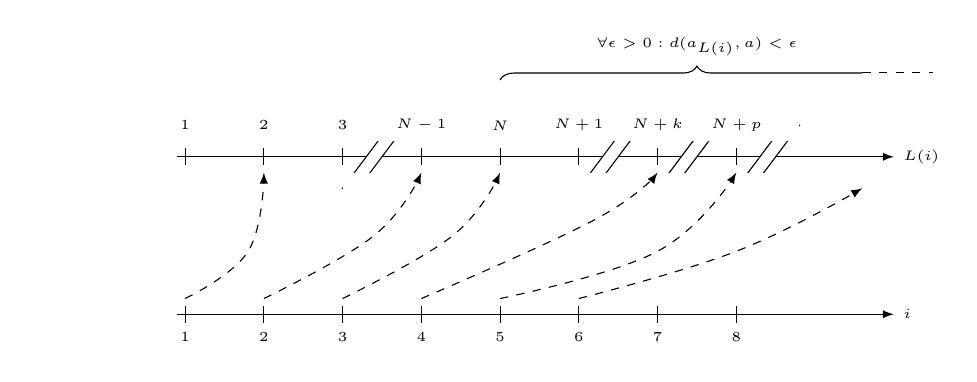
\begin{tikzpicture}
%\path [draw=black, fill=black] (-2,0) circle (2pt);
%\path [draw=black, fill=black, thick] (4,0.0) circle (2pt);
\draw[-latex] (0.,0) -- (10,0) ;
\foreach \x in  {0,...,8}{
\draw[shift={(\x,0)},color=black] (0pt,3pt) -- (0pt,-3pt);
};
\foreach \x in {0,...,2}
\draw[shift={(\x,0)},color=black] (0pt,0pt) -- (0pt,-3pt) ;

\draw[-latex] (0.,-2) -- (10,-2) ;
\foreach \x in  {0,...,8}
\draw[shift={(\x,-2)},color=black] (0pt,3pt) -- (0pt,-3pt);
\node[right] at (10,0) {\tiny$L(i)$};
\node[right] at (10,-2) {\tiny$i$};


\coordinate (v1) at (3,-0.4) {};
\coordinate (v2) at (3.2,-0.4) {};
\coordinate  (v3) at (3.8,0.4) {};
\coordinate (v4) at (3.6,0.4) {};
\draw[fill=white] (v1) -- (v2) -- (v3) -- (v4) --  cycle;
\coordinate (k1) at (6,-0.4) {};
\coordinate (k2) at (6.2,-0.4) {};
\coordinate  (k3) at (6.8,0.4) {};
\coordinate (k4) at (6.6,0.4) {};
\draw[fill=white] (k1) -- (k2) -- (k3) -- (k4) --  cycle;

\coordinate (p1) at (7.6,0.4) {} {} {};
\coordinate (p2) at (7,-0.4) {} {};
\coordinate (p3) at (7.2,-0.4) {} {};
\coordinate  (p4) at (7.8,0.4) {} {} {};
\draw[fill=white] (p1) -- (p2) -- (p3) -- (p4) --  cycle;
\coordinate (q1) at (8.6,0.4) {} {} {};
\coordinate (q2) at (8,-0.4) {} {};
\coordinate (q3) at (8.2,-0.4) {} {};
\coordinate  (q4) at (8.8,0.4) {} {} {} {};
\draw[fill=white] (q1) -- (q2) -- (q3) -- (q4) --  cycle;
\fill[white] (4,0.2)  rectangle (3.4,0.6);
\fill[white] (3,-0.2) rectangle (3.6,-0.6);
\fill[white] (6,0.2)  rectangle (6.8,0.6);
\fill[white] (5.8,-0.2) rectangle (6.4,-0.6);
\fill[white] (7,0.2)  rectangle (7.8,0.6);
\fill[white] (7.8,-0.2) rectangle (6.6,-0.6);
\fill[white] (8.2,0.2)  rectangle (8.8,0.6);
\fill[white] (8.8,-0.2) rectangle (7.8,-0.6);
\node at (1,0.4) {\tiny$1$};
\node at (2,0.4) {\tiny$2$};
\node at (3,0.4) {\tiny$3$};;
\node at (4,0.4) {\tiny$N-1$};;
\node at (5,0.4) {\tiny$N$};;
\node at (6,0.4) {\tiny$N+1$};;
\node at (7,0.4) {\tiny$N+k$};;
\node at (8,0.4) {\tiny$N+p$};;
\node (v5) at (1,-1.8) {};
\node (v7) at (2,-1.8) {};
\node (v9) at (3,-1.8) {};
\node (v11) at (4,-1.8) {};
\node (v13) at (5,-1.8) {};
\node (v15) at (6,-1.8) {};
\node at (1,-0.4) {};
\node (v6) at (2,-0.2) {};
\node (v8) at (4,-0.2) {};
\node at (5,-0.4) {};
\node (v10) at (5,-0.2) {};
\node (v12) at (7,-0.2) {};
\node (v14) at (8,-0.2) {};
\draw[dashed,-latex]  plot[smooth, tension=.7] coordinates {(v5) (1.8,-1.2) (v6)};
\draw[dashed,-latex]  plot[smooth, tension=.7] coordinates {(v7) (3.4,-1) (v8)};
\draw [dashed,-latex] plot[smooth, tension=.7] coordinates {(v9) (4.4,-1) (v10)};
\draw [dashed,-latex] plot[smooth, tension=.7] coordinates {(v11) (6.2,-0.8) (v12)};
\draw [dashed,-latex] plot[smooth, tension=.7] coordinates {(v13) (7,-1.2) (v14)};
\draw [dashed,-latex] plot[smooth, tension=.7] coordinates {(v15) (8,-1.2) (9.6,-0.4)};
\foreach \x in {0,...,8}
\draw[shift={(\x,-2)},color=black] (0pt,0pt) -- (0pt,-3pt) node[below] {\tiny$\x$};
\fill[white] (-1,0.5) rectangle (0.9,-2.5);
\draw [decorate,decoration = {brace,raise=5pt,
		amplitude=5pt,
		aspect=0.5}] (5,0.8) --  (10,0.8)node[pos=0.5,above=10pt,black]{\tiny$\forall\epsilon >0:d(a_{L(i)},a)<\epsilon$};;
\fill[white] (9.6,1.2) rectangle (10.2,0.6);

\draw[thin,dashed] (9.6,1.065) -- (10.5,1.065) ;
\end{tikzpicture}